%start preamble
\documentclass[paper=a4,fontsize=11pt]{scrartcl}%kind of doc, font size, paper size
\usepackage[ngerman]{babel}%for special german letters etc			
\usepackage[T1]{fontenc}%same as t1enc but better						
\usepackage[utf8]{inputenc}%utf-8 encoding, other systems could use others encoding
\usepackage{amsmath}%get math done
\usepackage{graphicx}%get pictures & graphics done
\graphicspath{{pictures/}}%folder to stash all kind of pictures etc
\usepackage{amssymb}%symbolics for math
\usepackage{amsfonts}%extra fonts
\usepackage{caption}%captions under everything
\usepackage{listings}
\usepackage[titletoc]{appendix}
\numberwithin{equation}{section} 
\usepackage{float}%for garphics and how to let them floating around in the doc
\usepackage{xcolor}%nicer colors, here used for links
\usepackage{dsfont}
\usepackage{geometry}
\usepackage{hyperref}
\usepackage{fancyhdr}
\usepackage{multicol}
\usepackage{xcolor}%nicer colors, here used for links

%settings colors for links
\hypersetup{
    colorlinks,
    linkcolor={blue!50!black},
    citecolor={blue},
    urlcolor={blue!80!black}
}

\definecolor{pblue}{rgb}{0.13,0.13,1}
\definecolor{pgreen}{rgb}{0,0.5,0}
\definecolor{pred}{rgb}{0.9,0,0}
\definecolor{pgrey}{rgb}{0.46,0.45,0.48}

\pagestyle{fancy}
\lhead{Netzwerke Übung (SoSe 2019)}
\rhead{FB 4 -- Angewandte Informatik\\ HTW-Berlin}
\lfoot{Übungsblatt 05 -- Routing \& Application Layer}
\cfoot{}
\fancyfoot[R]{\thepage}
\renewcommand{\headrulewidth}{0.4pt}
\renewcommand{\footrulewidth}{0.4pt}

\lstdefinestyle{Bash}{
  language=bash,
  showstringspaces=false,
  basicstyle=\small\sffamily,
  numbers=left,
  numberstyle=\tiny,
  numbersep=5pt,
  frame=trlb,
  columns=fullflexible,
  backgroundcolor=\color{gray!20},
  linewidth=0.9\linewidth,
  %xleftmargin=0.5\linewidth
}

\newlength\labelwd
\settowidth\labelwd{\bfseries viii.)}
\usepackage{tasks}
\settasks{counter-format =tsk[a].), label-format=\bfseries, label-offset=3em, label-align=right, label-width
=\labelwd, before-skip =\smallskipamount, after-item-skip=0pt}
\usepackage[inline]{enumitem}
\setlist[enumerate]{% (
labelindent = 0pt, leftmargin=*, itemsep=12pt, label={\textbf{\arabic*.)}}}

\pdfpkresolution=2400%higher resolution

%%here begins the actual document%%
\newcommand{\horrule}[1]{\rule{\linewidth}{#1}} % Create horizontal rule command with 1 argument of height

\DeclareMathOperator{\id}{id}

\begin{document}
\begin{center}
\Large{\textbf{Übungsblatt 5 -- Dynamisches Routing, Traceroute \& Application Layer}}
\end{center}
Nachdem Sie nun komplexere Netzwerke aufgesetzt haben und den Verkehr Ihrer Netzwerke analysiert haben, betrachten wir in der kommenden Übung die dynamische Umsetzung des Routings, sowie die Anwendungsschicht. Viele dieser \emph{Application Layer}-Protokolle nutzen Sie bereits ohne es bewusst wahrgenommen zu haben. Da Sie als angehende Netzwerkprofis aber nicht nur daran interessiert sind Dinge zu nutzen, sondern deren Aufbau zu verstehen, soll mit der Übung zum Application-Layer diese Lücke ein Stück weit kleiner werden.

\begin{center}\Large{\textbf{Aufgabe A -- Routing \& Traceroute}}\end{center}\vskip0.2in
\begin{enumerate}
	\item Im wesentlichen gibt es zwei fundamentale Routing-Algorithmen. Dies sind das Distanz-Vektor- und Link-State-Routing. Diese ermöglichen es den kürzesten Weg durch einen Graphen zu finden (Shortest-Path-Problem).\\
	Für gewöhnlich wird für das Distanz-Vektor-Routing der Bellman-Ford-Algorithmus verwandt, das Link-State-Routing nutzt den Dijkstra-Algorithmus.
	\begin{tasks}(1)
		\task Recherchieren Sie wie das Link-State-Routing unter Nutzung des Dijkstra-Algorithmus funktioniert.
		\task Recherchieren Sie wie das Distanz-Vektor-Routing unter Nutzung des Bellman-Ford-Algorithmus funktioniert.
		\task In welchen Protokollen finden diese beiden Protokollen Verwendung? Ist diesen Protokollen etwas gemein?
		\task \textbf{Fakultativ:} Warum wird keines der beiden Verfahren für das Exterior-Gateway-Protokoll (EGP) genutzt?
		\task Erläutern Sie die fundamentalen Unterschiede beider Lösungsansätze.
		\task Diskutieren Sie ob der Bellman-Ford-Algorithmus für das Link-State-Routing und der Dijkstra-Algorithmus für das Distanz-Vektor-Routing genutzt werden könnte.
	\end{tasks}
	\item Gegeben sei folgender Graph:
	\begin{figure}[H]
		\centering
		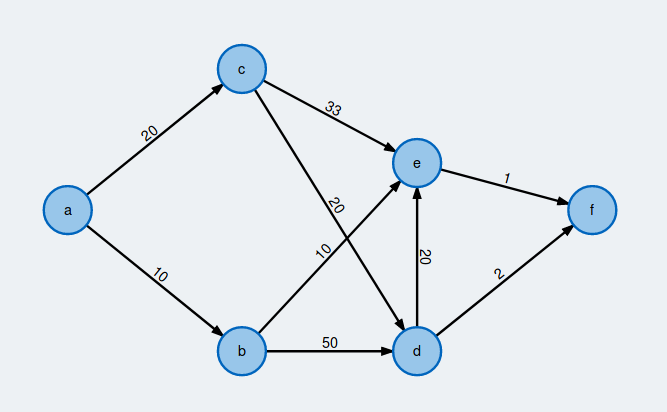
\includegraphics[scale=0.4]{dijkstra_example}
	\end{figure}
	Finden Sie den kürzesten Weg vom Knoten $a$ zum Knoten $f$!
	\begin{tasks}(1)
		\task Nutzen Sie zunächst den Dijkstra-Algorithmus.
		\task Anschließend soll der Bellman-Ford-Algorithmus genutzt werden. 
	\end{tasks}
\end{enumerate}

\begin{center}\Large{\textbf{Aufgabe B -- Traceroute}}\end{center}\vskip0.2in
\begin{enumerate}
	\item Lesen Sie die folgenden Artikel:\\
	\url{https://en.wikipedia.org/wiki/Traceroute},\\
	\url{https://linux.die.net/man/8/traceroute}.\\
	Beantworten Sie anschließend folgende Fragen:
	\begin{tasks}(1)
		\task Wofür wird Traceroute genutzt?
		\task Wie wird Traceroute umgesetzt, d.h. wie läuft eine \glqq Routen-Verfolgung\grqq\ ab?
		\task Welche Limitationen ergeben sich aus der Umsetzung?
		\task Dokumentieren Sie die Syntax, sowie die Bedeutung von Traceroute beispielhaft.
	\end{tasks}
	\item Lesen Sie folgendes Paper zu Paris-Traceroute von der ACM International Measurement Conference 2006:\\
	\url{http://conferences.sigcomm.org/imc/2006/papers/p15-augustin.pdf}
	\begin{tasks}(1)
		\task Warum ist eine \glqq neue\grqq\ Traceroute-Applikation notwendig?
		\task Nennen Sie drei Topologie-Anomalien die durch Paris-Traceroute erkannt werden können.
		\task Recherchieren Sie wie \emph{paris-traceroute} zu nutzen ist! Notieren Sie sich entsprechen die Kommandos und deren Bedeutung.
	\end{tasks}
\end{enumerate}

\begin{center}\Large{\textbf{Aufgabe B -- Domain Name System (DNS)}}\end{center}\vskip0.2in
Das Domain Name System ist ein dezentrales System (verteilte Datenbank nach der Client-Server-Architektur), dessen primäre Aufgabe die Adressauflösung von Domain Name(n) zu IP-Adresse(n) ist. M.a.W. DNS bietet eine Abbildung von Domainname auf IP-Adresse \footnote{Bzw. als Inverse -- die Abbildung von IP-Adresse auf Domainnamen (Reverse-Lookup)}.\\
In der dritten Übung wurde das DNS bereits kurz angeschnitten, da Ihre Netzwerke im letzten Schritt einen Uplink ins Internet erhalten haben und auch Domain Namen auflösen konnten.\\
Nun schauen wir uns das DNS und einige Tools etwas genauer an.
\begin{enumerate}
	\item Rekapitulieren Sie Ihr Wissen zu DNS!
	\begin{tasks}(1)
		\task Auf welchem Layer des OSI-Modells arbeitet DNS?
		\task Welches Transportprotokoll nutzt DNS?
		\task Auf welchem Port laufen DNS-Server standardmäßig?
	\end{tasks}
	\item Nennen und Erklären Sie die Komponenten des DNS-Systems.
	\begin{tasks}(1)
		\task Was ist gemeint wenn von einem Client-Server-Modell die Rede ist?
		\task Was wird unter dem Begriff DNS-Resolver verstaden?
		\task Was ist ein DNS-Root-Server, was ist ein TLD-Server und was ein Domain-Server?
		\task Was wird unter dem Konzept der Domain und was unter einer Zone verstanden?
		\task Was ist ein Stub im Kontext von DNS?
		\task Was ist ein Bind-Server?
		\task Recherchieren Sie welche wichtigen Ressource-Types DNS kennt.
	\end{tasks}
	\item Erläutern Sie die Auflösung einer DNS-Anfrage.
	\begin{tasks}
		\task Welche beiden Möglichkeiten einer Namensauflösung gibt es? Wie kann eine Name aufgelöst werden?
		\task Wie erfolgt die jeweilige Auflösung eines DNS-Requests?
		\task Verdeutlichen Sie sich anhand eines Beispiels, wie ein DNS-Request bearbeitet wird.
		\task DNS bietet theoretisch eine rekursive und iterative Namensauflösung, praktisch wird eine Mischung aus beiden Verfahren angewandt. Recherchieren Sie, wie diese Auflösung aussieht.
	\end{tasks}
	\item Recherchieren Sie kurz wie die Tools
	\begin{multicols}{3}
	\begin{itemize}
	\item host
	\item dig
	\item nslookup.
	\end{itemize}
	\end{multicols}
	zu nutzen sind.
	\begin{tasks}(1)
		\task Erläutern Sie kurz was jedes der oben genannten Tools leistet.
		\task Nennen Sie für jedes Tool geeignete Einsatzgebiete/ Szenarien.
		\task Recherchieren Sie die Syntax, sowie Semantik der Tools.
		\task Notieren und kommentieren Sie sich entsprechende Beispiele. 
	\end{tasks}
\end{enumerate}

\begin{center}\Large{\textbf{Aufgabe C -- HTTP(S) \& HTML}}\end{center}\vskip0.2in
Kein anderes Protokoll ist für das World-Wide-Web so wichtig wie \emph{HTTP}. In diesem Teil sollen Sie recherchieren, wie die bunten Seiten in Ihren Browser kommen.
\begin{enumerate}
	\item Recherchieren Sie zunächst was \emph{HTTP} ist.\\
	Eine gute Anlaufstelle wäre Tanenbaums Computer Networks Chapter 7.3 -- The World Wide Web. Jede andere Quelle ist ebenso gut!
	\item Erläutern Sie die Funktionswiese von \emph{HTTP}.
	\item Auf welcher Schicht des OSI-Modells ordnen Sie \emph{HTTP} ein?
	\item Auf welchen Port laufen meistens Webserver? Auf welchem Port läuft die verschlüsselte Variante \emph{HTTPs}?
	\item Wie sieht ein typischer \emph{HTTP}-Header aus?
	\item Nennen Sie alle \emph{HTTP}-Methoden. Notieren Sie sich was diese machen und wie deren Aufruf aussieht.
	\item Mittlerweile gibt es unterschiedliche Versionen von \emph{HTTP}. Vornehmlich sind dies $1.1$ und $HTTP/2$ -- nennen Sie einige fundamentale Unterschiede.
	\item Machen Sie sich kurz klar, welche Aufgabe SSL/TLS übernimmt.\\
	(Hinweis: An dieser Stelle genügt ein grobes Verständnis!)
	\item Recherchieren Sie wie die Tools \emph{telnet}, \emph{netcat} und \emph{openssl s\_client} für das Abfragen von \emph{HTTP} genutzt werden können.\\
	Wie sieht die Syntax zum Verbinden auf einen Server aus? Notieren Sie sich entsprechend Beispiele. Sie sollten als Vorbereitung auf die Laborübung sich auch das dazugehörige Arbeitsblatt anschauen, sodass Sie zielgerichtet nach entsprechenden Beispielen suchen können.
	\item Optional: Suchen Sie sich ein Tutorial zu \emph{openssl s\_client} heraus. Durchlaufen Sie entsprechendes Tutorial. \\
	Bspw.: \url{https://tinyurl.com/y9nnaz6a}
	\item Recherchieren Sie was \emph{STARTTLS} bedeutet. Worin unterscheidet sich \emph{STARTTLS} von \emph{HTTPs}?
	\item Recherchieren Sie kurz was ein kryptografisches Zertifikat ist. Wozu werden diese im Zusammenhang mit \emph{HTTPs} genutzt?
	\item Erläutern Sie wie Sie sich Zertifikate mit \emph{openssl} anschauen können.  
\end{enumerate}

\begin{center}\Large{\textbf{Aufgabe D -- E-Mail mit POP3, IMAPv4 \& SMTP}}\end{center}\vskip0.2in
Das Simple Mail Transfer Protokoll (SMTP) wird, wie der Name schon sagt, zum Austausch von E-Mails in Computernetzwerken genutzt. Primär wird es zum Weiterleiten von Mails zwischen Server genutzt. Auf Ihren Endgeräten kommt zumeist \emph{IMAP} oder \emph{POP3} zum Einsatz. 
\begin{enumerate}
	\item Recherchieren Sie zunächst was sich hinter den Akronymen POP3, IMAPv4, sowie SMTP verbirgt.
	\item Erläutern Sie im groben welche Aufgaben die oben genannten Protokolle übernehmen.
	\item Auf welcher Ebene des OSI-Modells arbeiten die Protokolle?
	\item Machen Sie sich im groben klar, wie diese Protokolle arbeiten.	
	\item Worin unterscheiden sich POP3 und IMAP?
	\item Auf welchen Ports arbeiten die drei Protokolle?
	\item Auf welchen Ports arbeiten die drei Protokolle mit Verschlüsselung?
	\item Recherchieren Sie wie IMAP, POP3 und SMTP via Kommandozeile genutzt werden können. Notieren Sie sich entsprechende Kommandos, sowie deren Bedeutung!
\end{enumerate}
\end{document}
